La titolazione è una tipica operazione dell'analisi chimica che consiste nel determinare la concentrazione o \textbf{titolo} di una specie chimica in soluzione, facendola reagire con una quantità nota di un dato reagente, detto \textbf{titolante}.
\subsection{Titolazione acido forte-base forte}
Si versa in un beker dell'acido, si aggiungono una o al massimo due gocce di una soluzione di una soluzione che per ora chiamiamo \textit{indicatore}, che è un composto che cambia colore nell'istante in cui si passa da un PH ad un altro. Il cambio di colore prende il nome di \textit{viraggio dell'indicatore}.

Ci sono vari tipi di indicatore. Se volessimo osservare la fine della titolazione, ossia partiamo da una soluzione acida e aggiungiamo una base, è utile un indicatore che abbia un punto di viraggio per pH pari a 7. Non è necessario che l'indicatore cambi colore esattamente a quel pH, perché ci sarà un valore di pH acido superato il quale con appena qualche goccia di base si raggiunge l'equivalenza. Gli indicatori sono dunque delle sostanze che in modo visibile ai nostri occhi cambiano colore e ci danno indicazione sul cambiamento di pH.

Nello specifico, questa reazione conviene farla usando come indicatore una sostanza chiamata \textit{fenoltaleina}, o meglio soluzioni estremamente diluite (all'1\%) di questa. Basta mettere una goccia di questa soluzione nel beker per potere osservare un cambio di colore pressoché immediato. Quando?

In ambiente acido è incolore (quindi ad esempio partendo da una soluzione di acido cloridrico non vedremmo nulla), per pH tra 8.5 e 9 da incolore diventa rossa, quindi avremo l'indicazione che il pH ha raggiunto tale valore al cambio di colore della soluzione. Se avessimo voluto capire invece quando si aveva l'equivalenza (cioè pH=7), potremmo pensare di aver perso questo punto di equivalenza. Vedremo che non è così: in prossimità del punto di equivalenza il pH varierà in modo repentino, con piccolissime aggiunte; al contrario, quando si è lontani dal punti di equivalenza il pH cambierà molto poco pur aggiungendo, se partiamo da una soluzione acida, parecchia base. D'altronde, avendo definito il pH come il logaritmo dell'inverso della concentrazione degli ioni $\rm H_3O^+$ di una soluzione, ci aspettiamo un andamento logaritmico e non lineare per il pH dopo l'aggiunta di una base.

\vspace{0.2cm}Immaginiamo di avere due soluzioni in due bekere diversi. Nel primo abbiamo 100 mL di HCl 0.1-N (nota: per l'HCl normalità e molarità coincidono). Aggiungiamo in esso la prima goccia di indicatore e poi aggiungiamo lentamente NaOH 0.1-N\footnote{Ovviamente non è necessario scegliere stesse concentrazioni, le usiamo per comodità di calcolo.}. In questo caso, se partiamo da 100 mL di acido cloridrico 0.1-N, quando avremo aggiunto 100 mL di idrossido di sodio 0.1-N (quindi stessi volumi e stesse concentrazioni) non avremo più né acido né base perché si saranno neutralizzati totalmente formando cloruro di sodio:

$$\ce{HCl(aq) + NaOH(aq) -> NaCl(aq) + H_2O}$$

Va da ricordare che HCl acquoso, visto che si tratta di un acido forte, significa ione $\rm H_3O^+$ e ione $\rm Cl^-$ totalmente dissociati. Analogamente NaOH acquoso, visto che si tratta di una base forte, significa ione $\rm Na^+$ e ione $\rm OH^-$ totalmente dissociati. Ma anche il cloruro di sodio, essendo un sale e quindi un elettrolita forte, sarà totalmente dissociato in $\rm Na^+$ e $\rm Cl^-$. Ne segue che l'unica vera reazione che sta venendo è la formazione di acqua: lo ione $\rm H^+$ dell'acido cloridrico e lo ione $\rm OH^-$ dell'NaOH danno luogo ad $\rm H_2O$, mentre gli altri ioni restano dissociati prima e dopo la reazione.

Quant'è il pH della soluzione iniziale?

Innanzitutto scriviamo sopra la reazione le quantità iniziali, sotto quelle finali.

All'inizio avevamo 100 mL di HCl 0.1N, il che significa (in questo caso in cui moli ed equivalenti coincidono) 0.1 moli in un litro di soluzione, quindi per sapere quante moli/equivalenti abbiamo in 1 mL dobbiamo dividere per 1000.

Per sapere gli equivalenti totali dobbiamo fare

$$\frac{0.1}{1000} \cdot 100$$

Per avere il pH del primo punto non è necessario nemmeno questo calcolo perché abbiamo già la concentrazione. Infatti il pH è definito come

$$\rm pH=\log \frac{1}{[H_3O^+]}$$

Va da ricordare che l'acido cloridrico in acqua darà luogo a ioni $\rm H_3O^+$ e ioni $\rm Cl^-$:

$$\ce{HCl + H_2O -> H_3O^+ + Cl^-}$$

Essendo un acido forte, tale reazione è compiuta da tutto l'acido. Ne segue che la concentrazione degli ioni $\rm H_3O^+$ corrisponde alla concentrazione dell'acido cloridrico.

$\rm [H_3O^+]$ è espressa come equivalenti/litro, che abbiamo già. Quindi il pH sarà

$$\rm pH=\log\frac{1}{0.1}=\log10=1$$

Quindi ancora prima di iniziare l'aggiunta della base abbiamo una soluzione che ha pH pari a 1.

A questo punto facciamo la prima aggiunta. Queste vanno fatte lentamente, quindi inizialmente aggiungiamo 10 mL di base. Dopo averli aggiunti calcoliamo il pH.

Torniamo alla reazione. Gli equivalenti iniziali di HCl erano 0.01 eq. Quanti equivalenti/moli ci sono in 10 mL di base?

Il calcolo è lo stesso.

$$\frac{0.1}{1000} \cdot 10=10^{-3}=0.001 \; eq$$

\begin{center}
    \begin{tabular}{ccccccc}
        0.01 &  & 0.001 & & / & &\\
        HCl & + & NaOH & \ce{->} & NaCl & + & $\rm H_2O$\\
        0.009 &  &  / & & 0.001 & &\\
    \end{tabular}
\end{center}

Calcoliamo la concentrazione di questa soluzione.

Non abbiamo base, abbiamo solo l'acido di cui ci sono $9 \cdot 10^{-3}$ moli. Esse stanno in un volume di 110 mL, quindi la molarità (e dunque la normalità) sarà data da

$$M=9 \cdot 10^{-3} \, \frac{1000}{110}=8.1818 \cdot 10^{-2}$$

Questa è la molarità della soluzione acida, perché la base è scomparsa e abbiamo solo acido cloridrico. Il calcolo da fare sarà allora

$$\rm pH=\log\left( \frac{1}{8.1818 \cdot 10^{-2}} \right)=1.09$$

A questo punto aggiungiamo 20 mL di NaOH, considerando però la quantità di acido di partenza.

Calcoliamo le moli di NaOH

$$n=\frac{0.1}{1000}\cdot 20=2 \cdot 10^{-3}$$

L'NaOH è in difetto e formerà 0.002 moli di sale. Di acido ce ne rimangono 0.008 moli

\begin{center}
    \begin{tabular}{ccccccc}
        0.01 &  & 0.002 & & / & &\\
        HCl & + & NaOH & \ce{->} & NaCl & + & $\rm H_2O$\\
        0.008 &  &  / & & 0.002 & &\\
    \end{tabular}
\end{center}

La molarità sarà

$$M=8\cdot 10^{-3} \, \frac{1000}{120}=6.6667 \cdot 10^{-2}$$

La soluzione è ancora acida, pertanto

$$\rm pH=\log\left( \frac{1}{6.6667 \cdot 10^{-2}} \right)=1.18$$

Adesso aggiungiamo 40 mL di base. Le moli di NaOH saranno $4 \cdot 10^{-3}$ (calcolate come prima), per cui la base continua ad essere in difetto, quindi viene neutralizzata totalmente, dando $4 \cdot 10^{-3}$ moli di sale. Ci restano 0.006 moli di acido:

\begin{center}
    \begin{tabular}{ccccccc}
        0.01 &  & 0.004 & & / & &\\
        HCl & + & NaOH & \ce{->} & NaCl & + & $\rm H_2O$\\
        0.006 &  &  / & & 0.004 & &\\
    \end{tabular}
\end{center}

La molarità sarà

$$M=6\cdot 10^{-3} \, \frac{1000}{140}=4.2857\cdot 10^{-2}$$

$$\implies \rm pH=\log\left( \frac{1}{4.2857 \cdot 10^{-2}} \right)=1.37$$

Aggiungiamo 50 mL di NaOH 0.1-N. A questo punto arriviamo a metà della titolazione. Si ottengono 0.005 moli di sale e restano 0.005 moli di acido

\begin{center}
    \begin{tabular}{ccccccc}
        0.01 &  & 0.005 & & / & &\\
        HCl & + & NaOH & \ce{->} & NaCl & + & $\rm H_2O$\\
        0.005 &  &  / & & 0.005 & &\\
    \end{tabular}
\end{center}

$$M=5 \cdot 10^{-3} \, \frac{1000}{150}=3.333 \cdot 10^{-2}$$

$$\implies \rm pH = \log \left( \frac{1}{3.333 \cdot 10^{-2}} \right)=1.48$$

Notiamo che, pur avendo neutralizzato metà dell'acido di partenza, il pH non è aumentato nemmeno di mezza unità.

\vspace{0.2cm}Calcoliamo il pH dopo aver aggiunto 80 mL di base.

Abbiamo aggiunto 0.008 equivalenti/moli di base, che sono ancora in difetto, quindi vanno via producendo 0.008 moli di sale e ci restano 0.002 moli di acido:

\begin{center}
    \begin{tabular}{ccccccc}
        0.01 &  & 0.008 & & / & &\\
        HCl & + & NaOH & \ce{->} & NaCl & + & $\rm H_2O$\\
        0.002 &  &  / & & 0.008 & &\\
    \end{tabular}
\end{center}

La molarità dell'acido sarà

$$M=2 \cdot 10^{-3} \, \frac{1000}{180}=1.1111 \cdot 10^{-2}$$

$$\implies \rm pH = \log \left( \frac{1}{1.1111 \cdot 10^{-2}} \right)=1.95$$


Aggiungiamo 90 mL di base, che significa 0.009 moli. Essendo in difetto, l'NaOH va tutto via e dà 0.009 moli di sale e restano 0.001 moli di acido:

\begin{center}
    \begin{tabular}{ccccccc}
        0.01 &  & 0.009 & & / & &\\
        HCl & + & NaOH & \ce{->} & NaCl & + & $\rm H_2O$\\
        0.001 &  &  / & & 0.009 & &\\
    \end{tabular}
\end{center}

La concentrazione è

$$M=1 \cdot 10^{-3} \, \frac{1000}{190}=5.2632 \cdot 10^{-3}$$

$$\implies \rm pH = \log \left( \frac{1}{5.2632 \cdot 10^{-3}} \right)=2.28$$

Aggiungiamo adesso 95 mL, cioè $9.5 \cdot 10^{-3}$ moli di base, che sono in difetto e producono $9.5 \cdot 10^{-3}$ moli di sale. Restano $5 \cdot 10^{-4}$ moli di acido.

\begin{center}
    \begin{tabular}{ccccccc}
        0.01 &  & $9.5 \cdot 10^{-3}$  & & / & &\\
        HCl & + & NaOH & \ce{->} & NaCl & + & $\rm H_2O$\\
        $5 \cdot 10^{-4}$ &  &  / & & $9.5 \cdot 10^{-3}$ & &\\
    \end{tabular}
\end{center}

$$M=5 \cdot 10^{-4} \, \frac{1000}{195}=2.5641 \cdot 10^{-3}$$

$$\implies \rm pH=\log \left( \frac{1}{2.5641 \cdot 10^{-3}} \right)=2.59$$

Andiamo a 99 mL. Avremo $9.9 \cdot 10^{-3}$ moli di base e quindi $1.0 \cdot 10^{-4}$ moli di acido

\begin{center}
    \begin{tabular}{ccccccc}
        0.01 &  & $9.9 \cdot 10^{-3}$  & & / & &\\
        HCl & + & NaOH & \ce{->} & NaCl & + & $\rm H_2O$\\
        $1 \cdot 10^{-4}$ &  &  / & & $9.9 \cdot 10^{-3}$ & &\\
    \end{tabular}
\end{center}

$$M=1.0 \cdot 10^{-4} \, \frac{1000}{199}=5.0251\cdot 10^{-4}$$

$$\implies \rm pH=\log \left( \frac{1}{5.0251\cdot 10^{-4}} \right)=3.30$$

Aggiungiamo 99.5 mL. Le moli di base saranno $9.95 \cdot 10^{-3}$. Siamo ancora in difetto, quindi avremo $9.95 \cdot 10^{-3}$ moli di sale e restano $5 \cdot 10^{-5}$ moli di acido

\begin{center}
    \begin{tabular}{ccccccc}
        0.01 &  & $9.95 \cdot 10^{-3}$  & & / & &\\
        HCl & + & NaOH & \ce{->} & NaCl & + & $\rm H_2O$\\
        $5 \cdot 10^{-5}$ &  &  / & & $9.95 \cdot 10^{-3}$ & &\\
    \end{tabular}
\end{center}

$$M=5.0 \cdot 10^{-5} \, \frac{1000}{199.5}=2.5063 \cdot 10^{-4}$$

$$\implies \rm pH=\log \left( \frac{1}{2.5063 \cdot 10^{-4}} \right)=3.60$$

Aggiungiamo 99.9 mL. Le moli di base saranno $9.99 \cdot 10^{-3}$. La base continua ad essere in difetto e produrrà $9.99 \cdot 10^{-3}$ moli di sale. Resteranno $1 \cdot 10^{-5}$ moli di acido

\begin{center}
    \begin{tabular}{ccccccc}
        0.01 &  & $9.99 \cdot 10^{-3}$  & & / & &\\
        HCl & + & NaOH & \ce{->} & NaCl & + & $\rm H_2O$\\
        $1 \cdot 10^{-5}$ &  &  / & & $9.99 \cdot 10^{-3}$ & &\\
    \end{tabular}
\end{center}

$$M=1 \cdot 10^{-5} \, \frac{1000}{199.9}=5.0025 \cdot 10^{-5}$$

$$\implies \rm pH=\log \left( \frac{1}{5.0025 \cdot 10^{-5}} \right)=4.30$$

Gli strumenti che usiamo per aggiungere la base si chiamano burette. Esse hanno la precisione di 0.1 mL. Il loro rubinetto può però essere aperto in modo tale da fare scendere goccia a goccia la soluzione e le burette sono tali che 1 mL contenga 1/20 di mL, ossia il volume di una goccia è 0.05 mL.

Aggiungiamo quindi come volume della base 99.95 mL. Avremo $9.995 \cdot 10^{-3}$ moli di base e quindi anche di sale perché non abbiamo eccesso di base. Restano poi $5 \cdot 10^{-6}$ moli di acido:

\begin{center}
    \begin{tabular}{ccccccc}
        0.01 &  & $9.995 \cdot 10^{-3}$  & & / & &\\
        HCl & + & NaOH & \ce{->} & NaCl & + & $\rm H_2O$\\
        $5 \cdot 10^{-6}$ &  &  / & & $9.995 \cdot 10^{-3}$ & &\\
    \end{tabular}
\end{center}

$$M=5 \cdot 10^{-6} \, \frac{1000}{199.95}=2.5006 \cdot 10^{-5}$$

$$\implies \rm pH=\log \left( \frac{1}{2.5006 \cdot 10^{-5}} \right)=4.60$$

Ci resta l'ultima goccia per la neutralizzazione totale, cioè aggiungiamo 100 mL di base

\begin{center}
    \begin{tabular}{ccccccc}
        0.01 &  & 0.01  & & / & &\\
        HCl & + & NaOH & \ce{->} & NaCl & + & $\rm H_2O$\\
        / &  & / & & 0.01 & &\\
    \end{tabular}
\end{center}

A questo punto la concentrazione degli ioni $\rm H_3O^+$, ossia la molarità, qual è? Non abbiamo più né acido né base e il cloruro di sodio è un sale neutro, pertanto sarà quella dell'autodissociazione dell'acqua:

$$\rm [H_3O^+]=10^{-7} \implies pH=7$$

\vspace{0.2cm}A questo punto riportiamo i valori del pH e dei mL di base in una tabella:

\vspace{0.7cm}\begin{center}
    \begin{tabular}{|p{1.5cm}|p{1.5cm}||p{1.5cm}|p{1.5cm}|}
        \textbf{pH} & \textbf{mL} & \textbf{pH} & \textbf{mL}\\
        1 & 0 & 2.59 & 95\\
        1.09 & 10 & 3.30 & 99\\
        1.18 & 20 & 3.60 & 99.5\\
        1.37 & 40 & 4.30 & 99.9\\
        1.48 & 50 & 4.60 & 99.95\\
        1.95 & 80 & 7 & 100\\
        2.28 & 90 &&\\
    \end{tabular}
\end{center}

\newpage

Notiamo che all'inizio il pH cambiava pochissimo: 10 mL fanno variare il pH di meno di 0.1; 20 mL di meno di 0.2; 40 mL di meno di 0.4 e 50 mL meno di 0.5. Quando siamo arrivati a 90 mL abbiamo superato il valore di 2, perché con 80 mL il pH valeva ancora 1.95. Tra 95 mL e 99 mL, cioè 4 mL in più, il pH cambia da 2.28 a 2.59, infatti ci stiamo avvicinando alla salita logaritmica. Infine quando mancano due gocce alla neutralità il pH è 4.30, quando ne manca solamente una il pH è 4.60 e dopo avere aggiunto pure l'ultima goccia il pH è 7.

Notiamo che serve molta precisione, quindi conviene usare 4 cifre dopo la virgola approssimando la quarta cifra dopo aver letto la quinta.

Continuiamo: aggiungiamo un'ulteriore goccia, quindi si hanno 100.05 mL di base, ossia una goccia in più rispetto alla neutralità. Avremo $(0.1 \cdot 100.05)/1000=1.0005 \cdot 10^{-2}$ moli di base, che è in eccesso. Quindi stavolta l'acido cloridrico va via del tutto e produce 0.01 moli di sale. Resta $5 \cdot 10^{-6}$ moli di base:

\begin{center}
    \begin{tabular}{ccccccc}
        0.01 &  & $1.0005 \cdot 10^{-2}$ & & / & &\\
        HCl & + & NaOH & \ce{->} & NaCl & + & $\rm H_2O$\\
        / &  &  $5 \cdot 10^{-6}$ & & 0.01 & &\\
    \end{tabular}
\end{center}

La molarità sarà, calcolata rispetto all'NaOH:

$$M=5 \cdot 10^{-6} \, \frac{1000}{200.5}=2.4993 \cdot 10^{-5}$$

Avendo una base dobbiamo calcolare il pOH:

$$\rm pOH = \log \left( \frac{2}{2.4993 \cdot 10^{-5}} \right)=4.6$$

$$\implies \rm pH=14 - pOH=14-4.6=9.40$$

Va da notare che con due gocce abbiamo avuto un salto di 6 unità di pH, ciò perché siamo in prossimità dell'equivalenza. Infatti lontano da essa sono serviti 90 mL di base per portare il pH da 1 a 2, qua invece abbiamo usato solo 0.1 mL.

Aggiungiamo un'altra goccia di base, cioè 100.1 mL di base

$$n_{\text{NaOH}}=\frac{0.1 \cdot 100.1}{1000}\approx 0.01001\implies n_{\text{HCl}}=0.01001-0.01 = 1 \cdot 10^{-5}$$

$$M=1 \cdot 10^{-5} \, \frac{1000}{200.1}=4.9975 \cdot 10^{-5}$$

$$\rm pOH=\log \left( \frac{1}{4.9975 \cdot 10^{-5}} \right)=4.30 \implies \rm pH=14-4.30=9.70$$

Aggiungiamo 110 mL di titolante

$$n_{\text{NaOH}}=\frac{0.1 \cdot 110}{1000}= 0.011\implies n_{\text{HCl}}=0.011-0.01 = 1 \cdot 10^{-3}$$

$$M=1 \cdot 10^{-3} \, \frac{1000}{210}=4.7619 \cdot 10^{-3}$$

$$\rm pOH=\log \left( \frac{1}{4.7619 \cdot 10^{-3}} \right)=2.32 \implies \rm pH=14-2.32=11.67$$

Aggiungiamo 120 mL di titolante

$$n_{\text{NaOH}}=\frac{0.1 \cdot 120}{1000}= 0.012\implies n_{\text{HCl}}=0.012-0.01 = 2 \cdot 10^{-3}$$

$$M=2 \cdot 10^{-3} \, \frac{1000}{220}=9.0909 \cdot 10^{-3}$$

$$\rm pOH=\log \left( \frac{1}{9.0909 \cdot 10^{-3}} \right)=2.04 \implies \rm pH=14-2.04=11.96$$

Aggiungiamo 150 mL di titolante

$$n_{\text{NaOH}}=\frac{0.1 \cdot 150}{1000}= 0.015\implies n_{\text{HCl}}=0.015-0.01 = 5 \cdot 10^{-3}$$

$$M=5 \cdot 10^{-3} \, \frac{1000}{250}=2 \cdot 10^{-2}$$

$$\rm pOH=\log \left( \frac{1}{2 \cdot 10^{-2}} \right)=1.69 \implies \rm pH=14-1.69=12.31$$

Se riportiamo i dati su un grafico avremo tale andamento:

\begin{figure}[H]
    \hspace{1.3cm}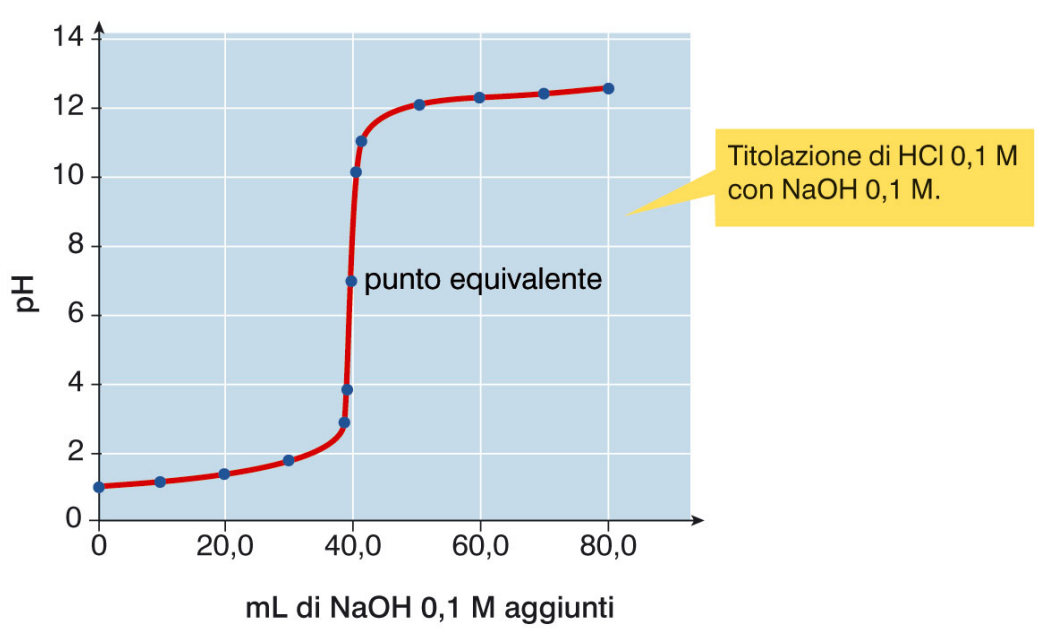
\includegraphics[width=14cm]{immagini/titolazione_acido_forte_base_forte.png}
\end{figure}

Per questa titolazione acido forte-base forte si ha il flesso per pH=7.

Se fossimo partiti al contrario da una base e avessimo aggiunto l'acido, il pH sarebbe stato alto all'inizio, variando inizialmente poco e bruscamente poi in prossimità dell'equivalenza per poi appiattirsi di nuovo.

A questo punto capiamo che qualunque indicatore abbia un intervallo di viraggio compreso nella regione in cui il pH varia velocemente è ottimo per i nostri scopi, perché avreo variazione di pH con poche gocce. Se inoltre sappiamo a priori quando l'indicatore vira (ad esempio la fenoltaleina vira tra 8.8 e 9), possiamo capire di quanto abbiamo ecceduto nell'aggiungere il titolante. Chiaramente bisogna essere pronti a chiudere il rubinetto appena vediamo la soluzione cambiare colore.

Sapendo quando l'indicatore vira possiamo capire quante gocce dobbiamo aggiungere o togliere per arrivare a pH pari a 7.

Affinché l'indicatore sia utile ai nostri scopi serve che il suo intervallo di viraggio sia nell'arco di 1-2 gocce.

A cosa serve questo discorso?

Se avessimo delle soluzioni di cui conosciamo precisamente la concentrazione questo lavoro non servirebbe. Se invece avessimo una soluzione di una data specie di cui non conosciamo la concentrazione, con questo metodo potremmo ottenerla, perché ciò che succede è che abbiamo un becher in cui c'è una certa quantità di una specie (acido o base che sia) e poi ne aggiungiamo un'altra, quindi conosciamo con esattezza i due volumi, quello della specie nel becher e quello che misuriamo goccia a goccia.
\subsection{Acidi deboli}
Come calcoliamo il pH di una specie che invece non è forte, cioè una specie di cui ne mettiamo una certa quantità ma se ne dissocia poca?

Nella reazione tra HCl e NaOH abbiamo utilizzato un criterio: la concentrazione degli ioni $\rm H_3O^+$ è uguale a quella dell'HCl in eccesso (o se eravamo a destra dell'equivalenza si assumeva la concentrazione degli ioni $\rm OH^-$ uguale a quella dell'NaOH in eccesso). Ciò non è più vero con un acido debole. L'esempio tipico è l'acido acetico:

$$\ce{CH_3COOH(aq) + H_2O <--> CH_3COO^-(aq) + H_3O^+(aq)}$$

L'acido acetico si dissocia poco, quindi avremo una reazione di equilibrio. La costante di questa dissociazione vale $1.8 \cdot 10^{-5}$, che per definizione si esprime come

$$k_a=\frac{\rm{[CH_3COO^-]} \cdot \rm{[H_3O^+]}}{\rm{[CH_3COOH]}}$$

Dal basso valore della costante deduciamo che si dissocia poco, ma quelle poche molecole che si dissociano producono uno ione acetato e uno ione $\rm H_3O^+$ ciascuna, quindi numericamente le due concentrazioni saranno sempre uguali. La costante si può allora scrivere come

$$k_a=\frac{\rm{[H_3O^+]^2}}{\rm{[CH_3COOH]}}$$

Nota: queste sono quantità all'equilibrio, non quelle di partenza. Ne segue che al denominatore abbiamo la concentrazione dell'acido acetico rimasto.

Essendosi l'acido dissociato molto poco, non commettiamo errore di calcolo, dato che il pH è dato con due cifre decimali, se facciamo l'approssimazione di immaginare che la concentrazione all'equilibrio sia uguale a quella di partenza. Tale approssimazione ci fa evitare un'equazione di secondo grado. Se infatti all'inizio avessimo ad esempio una mole di acido di cui se ne dissocia una quantità $x$, avremo $x$ moli di ione acetato e $x$ moli di $\rm H_3O^+$. Di acido ce ne restano $1-x$ moli:

\begin{center}
    \begin{tabular}{ccccccc}
        1 &  &  & & / & &\\
        $\rm CH_3COOH(aq)$ & + & $\rm H_2O$ & \ce{<-->} & $\rm CH_3COO^-(aq)$ & + & $\rm H_3O^+$\\
        $1-x$ & & & & $x$ & & $x$\\
    \end{tabular}
\end{center}

La costante allora diverrebbe $k=\frac{x^1}{1-x^2}$

Se invece partiamo da $c$ moli avremo
$$k_a = \frac{x^2 \, c^2}{(1-x)c}= c \frac{x^2}{(1-x)}$$

Se però trascuriamo $x$ al denominatore avremo

$$[\text{H}_3\text{O}^+]^2= k_a \cdot c_a \implies [\text{H}_3\text{O}^+] = \sqrt{k_a \cdot c_a}$$

con $c_a$ concentrazione iniziale dell'acido.

Quindi la concentrazione degli ioni $\rm H_3O^+$ è data dalla radice della costante di equilibrio dell'acido per la sua concentrazione. Ciò non avviene per gli acidi forti in cui la concentrazione dell'acido coincide con quella degli ioni $\rm H_3O^+$.

Facciamo un esempio di calcolo: immaginiamo di avere 0.12345 grammi di $\rm CH_3COOH$ sciolti in una soluzione di 500 mL. Calcoliamo innanzitutto la concentrazione: anche quest'acido è monoprotico, quindi normalità e molarità coincidono perché peso molecolare e peso equivalente coincidono, per cui

$$c_a=N=M=\frac{0.12345 \cdot 1000}{60.052 \cdot 500}$$

$$\implies [\text{H}_3\text{O}^+]=\sqrt{1.8 \cdot 10^{-5} \cdot \frac{0.12345 \cdot 1000}{60.052 \cdot 500}}=2.7204 \cdot 10^{-4}$$

$$\implies \rm pH=\log \left( \frac{1}{2.7204 \cdot 10^{-4}} \right)=3.57$$

Gli acidi deboli, a parità di concentrazione con un acido forte, danno un pH meno acido. 

\subsection{Basi deboli}

L'esempio classico di pH di basi deboli è il caso dell'ammoniaca $\rm NH_3$, che è un gas. Noi lavoriamo con le soluzioni ammoniacali, cioè facciamo gorgogliare questo gas disciogliendolo in acqua. Quello che succede è che si forma l'addotto $\rm NH_3 \cdot H_2O$, cioè ogni molecola di $\rm NH_3$ associa una molecola d'acqua. A volte si fa la somma algebrica e si scrive $\rm NH_4OH$, ma è meno corretta. Ciononostante si usa perché ci dà un'idea più diretta della dissociazione che avviene:

$$\ce{NH_4OH <--> NH_4^+ + OH^-}$$

Useremo la prima notazione:

$$\ce{NH_3 \cdot H_2O <--> NH_4^+ + OH^-}$$

Questa sarà la dissociazione di tale base debole. La relativa costante di dissociazione è

$$k_b= \frac{\rm{[NH_4^+] \cdot [OH^-]}}{\rm{[NH_3 \cdot H_2O]}}$$

Quanto detto per l'acido acetico vale anche per questa base: ogni molecola di ammoniaca che si dissocia produrrà uno ione ammonio $\rm NH_4^+$ e uno ione $\rm OH^-$, quindi le loro concentrazioni saranno numericamente sempre uguali, quindi ci basta prenderne una ed elevarla al quadrato:

$$k_b= \frac{\rm{[OH^-]^2}}{\rm{[NH_3 \cdot H_2O]}}$$

$$\implies \rm [OH^-] = \sqrt{ \textit{k}_{\textit{b}} \cdot [NH_3 \cdot H_2O]}$$

$$\implies  [\text{OH}^-] = \sqrt{ k_b \cdot c_b}$$ù

La costante di dissociazione dell'$\rm NH_3$ è pari a $1.8 \cdot 10^{-5}$, cioò significa che questa dissociazione ha un equilibrio spostato a sinistra, ossia l'ammoniaca si dissocia poco. Pertanto possiamo trascurare la quantità che si è dissociata e immaginare che all'equilibrio si abbia la concentrazione iniziale della base:

$$[\text{OH}]=\sqrt{k_b \cdot c_b}$$

In questo modo calcoliamo prima la concentrazione degli ioni $\rm OH^-$, poi il pOH e quindi il pH.

\vspace{0.2cm}Facciamo un esempio numerico: immaginiamo di avere 25 grammi di $\rm NH_3$ in un volume di 1 litro di soluzione finale. Attenzione! avremo 25 grammi della specie $\rm NH_3H_2O$, quindi il peso molecolare sarà circa 35. Dunque

$$[\text{OH}^-]=\sqrt{1.8 \cdot 10^{-5} \cdot \frac{25}{35}}=3.5857 \cdot 10^{-3}$$

$$\implies \rm pOH= \log \left( \frac{1}{3.5857 \cdot 10^{-3}} \right)=2.45 \implies pH=11.55$$

Abbiamo quindi visto che un'acido forte mostra un pH intorno ad 1, un acido debole un pH intorno a 3 (differenza notevole perché abbiamo a che fare con una scala logaritmica). Una base debole mostra pH superiore a 11. Tuttavia osservando le espressioni per acidi e basi deboli intuiamo che le concentrazioni sono fortemente determinate dalla costante di dissociazione. Ne segue che il pH delle speci deboli è fortemente determinato dalla costante. Facciamo questo confronto perché se avessimo la necessità di ottenere una soluzione con un dato pH dobbiamo sapere qual è la specie in grado di produrci tale pH, e per fare ciò si va a vedere il valore della costante di dissociazione.

\subsection{Reazioni di idrolisi}
Se mettiamo un cucchiaino di cloruro di sodio in acqua ciò che avviene è solo la dissociazione dell'NaCl in ione $\rm Na^+$ e $\rm Cl^-$, senza che questi subiscano reazioni successive:

$$\ce{NaCl(aq) -> Na^+(aq) + Cl^-(aq)}$$

Se anziché avere cloruro di sodio avessimo acetato di sodio $\rm CH_3COONa$ cosa succederebbe?

Questo composto in acqua si dissocia in ione acetato $\rm CH_3COO^-$ e ione $\rm Na^+$

$$\ce{CH_3COONa -> CH_3COO^-(aq) + Na^+(aq)}$$

Nota: mettiamo una singola freccia perché è un sale, e i sali solubili sono tutti elettroliti forti e pertanto totalmente dissociati.

Lo ione $\rm Na^+(aq)$ non darà luogo ad ulteriori reazioni perché in acqua si hanno ioni $\rm H_3O^+$ e ioni $\rm OH^-$. La specie NaOH non si potrà formare perché è una base forte quindi totalmente dissociata, cosa che porta lo ione $\rm Na^+$ e lo ione $\rm OH^-$ a non potersi riassociare.

Lo ione acetato $\rm CH_3COO^-$ invece è la base di un acido debole, per cui dà ulteriori reazioni. In particolare esso reagisce con una molecola d'acqua e dà un equilibrio (a differenza della prima reazione che è una dissociazione in cui non c'è equilibrio). Con tale reazione di equilibrio lo ione acetato strappa un protone all'acqua riformando l'acido acetico e lasciando ioni $\rm OH^-$

$$\ce{CH_3COO^-(aq) + H_2O <--> CH_3COOH(aq) + OH^-(aq)}$$

Si forma quindi un acido, ma la soluzione è basica. Queste reazioni sono dette di \textbf{idrolisi}, in particolare la reazione appena vista è detta \textbf{idrolisi basica}.

La soluzione sarà basica perché l'acido che si forma è indissociato, ma in soluzione abbiamo anche eccesso di ioni $\rm OH^-$.

Quello che sta succedendo è che mettiamo in acqua un sale che è neutro (l'acetato di sodio) e troviamo una soluzione che è basica. Questo discorso è tipico di tantissimi saponi: essi sono neutri finché sono lontani dall'acqua, ma appena li bagniamo la specie che si ottiene non è più neutra.

In sintesi: abbiamo messo in acqua un sale neutro, che essendo un elettrolita forte si dissocia totalmente, dando ione acetato e ione sodio. Quest'ultimo non fa nulla, resta $\rm Na^+(aq)$, ossia anche se ci sono ioni $\rm OH^-$ in soluzione non si avrà la formazione dell'NaOH perché quest'ultimo è una base forte, quindi è tutta dissociata e non può associarsi. Invece lo ione acetato che produciamo, che è la base coniugata di un acido debole, strappa un protone all'acqua, forma l'acido acetico e pertanto avremo un eccesso di ioni $\rm OH^-$.

Trattandosi di un equilibrio, scriviamo la costante di questo equilibrio $k_i$, che sta per \textit{costante di idrolisi}. Va da notare che potremmo scrivere $k_b$ perché abbiamo scoperto che l'acetato di sodio è una base, in quanto sviluppa un ambiente basico con eccesso di ioni $\rm OH^-$:

$$k_i = \rm{\frac{[CH_3COOH] [OH^-]}{[CH_3COO^-]}} \quad (*)$$

Tuttavia i testi non riportano questa costante, ma quella $k_a$ dell'acido acetico sì. Allora moltiplichiamo e dividiamo per la concentrazione degli ioni $\rm H_3O^+$:

$$k_i = \rm{\frac{[CH_3COOH] [OH^-]}{[CH_3COO^-]} \cdot \frac{[H_3O^+]}{[H_3O^+]}}$$

In tale espressione al numeratore compare il prodotto $\rm [OH^-] \cdot [H_3O^+]$, che è il prodotto ionico dell'acqua $k_w$ che vale $1.0 \cdot 10^{-14}$. Ciò che invece resta è uguale all'inverso della $k_a$ dell'acido acetico:

$$k_i = \frac{k_w}{k_a}$$

Torniamo adesso alla $(*)$. Se guardiamo la reazione di equilibrio ci accorgiamo che ogni ione acetato che si idrolizza produrrà una molecola di acido e uno ione $\rm OH^-$, ossia queste quantità saranno uguali, quindi possiamo scrivere una sola quantità al quadrato:

$$k_i = \rm{\frac{[OH^-]^2}{[CH_3COO^-]}} \implies [OH^-]= \sqrt{\textit{k}_\textit{i} \cdot [CH_3COO^-]}$$

cioè la concentrazione degli ioni $\rm OH^-$ è uguale alla radice di $k_i$ per la concentrazione dello ione acetato all'equilibrio.

Se però consideriamo la prima definizione di $k_i$ come il rapporto $k_w/k_a$, abbiamo che

$$k_i = \frac{k_w}{k_a} = \frac{10^{-14}}{1.8 \cdot 10^{-5}}=5.55 \cdot 10^{-10}$$

Quindi la costante della reazione di equilibrio è molto piccola. Ne segue che la reazione è spostata a destra quasi per niente, ovvero gli ioni acetato ad idrolizzarsi sono pochi:

$$\rm{\frac{[OH^-]^2}{[CH_3COO^-]}} \approx 5.55 \cdot 10^{-10}$$

\E allora lecito supporre che non si sia idrolizzato nessuno ione acetato e che quindi la concentrazione all'equilibrio è uguale alla concentrazione iniziale del sale di partenza (la concentrazione iniziale di ione acetato è uguale a quella iniziale del sale, dato che quest'ultimo si dissocia totalmente):

$$[\text{OH}^-]=\sqrt{k_i \cdot C_s}=\sqrt{\frac{k_w}{k_a}\cdot C_s}$$

\E quindi ribadito il fatto che la concentrazione degli ioni $\rm [OH^-]$ è determinata dal valore di $k_i$, e la concentrazione del sale influisce poco. Dunque a priori ci aspettiamo già certi valori di pOH, ossia visto che lo ione acetato che si riassocia è pochissimo avremo una scarsa produzione di ioni $\rm [OH^-]$, quindi ci aspettiamo un pH basso, vicino alla neutralità, circa 8.

Facciamo un esempio. Consideriamo 7.5432 grammi di acetato di sodio AcNa in 575 mL. avremo

$$\rm [OH^-]=\sqrt{\frac{1 \cdot 10^{-14}}{1.8 \cdot 10^{-5}}\cdot \frac{7.5432}{82.0343} \cdot \frac{1000}{575}}=9.425 \cdot 10^{-6}$$

$$\implies \rm pOH = \log \left( \frac{1}{9.425 \cdot 10^{-6}} \right)=5.03 \implies pH= 14-5.03=8.97$$
\subsubsection{Calcolare le moli conoscendo il volume ma non la massa}
Supponiamo di prelevare 3 litri di ammoniaca gassosa a condizioni normali e di farli gorgogliare in 700 mL di soluzione finale. Se la quantità ci viene data in litri e non in grammi come calcoliamo la concentrazione?

Ricordiamo la legge dei volumi molari, la quale afferma che a condizioni normali una mole di un gas occuperà sempre, qualunque sia il gas, un volume di 22.414 litri. Dato che siamo in condizioni normali, avremo

$$n_{\text{NH}_3}=\frac{3 \, L}{22.414 \, L}$$

ciò vale per qualunque gas prelevato a condizioni normali. Se venisse invece prelevato a condizioni diverse, conoscendo pressione e temperatura avremo che
$$n=\frac{PV}{RT}$$
\subsection{Soluzioni tampone}
Queste soluzioni si chiamano così perché hanno la caratteristica di mantenere un pH quasi invariato anche se noi dall'esterno, dopo aver generato la soluzione, aggiungiamo piccole quantità di acido o di base.

Va da ricordare che facendo la titolazione ad un certo punto con una goccia di base siamo passati da pH 4.6 a pH 7 e con un'altra goccia ancora a pH 9.4, quindi piccole quantità di acido o di base possono far cambiare drasticamente il pH. Chiaramente se anziché gocce mettiamo millilitri la situazione è ancora più marcata. Questo soluzioni tampone però hanno la caratteristica di fissare il pH a precisi valori e farlo variare pochissimo anche se aggiungiamo acido o base dall'esterno.

Sono importantissime perché esistono delle reazioni che avvengono a precisi valori di pH, quindi se tale reazione avviene in un ambiente opportuno procede, altrimenti no. Può darsi che man mano che queste reazioni procedono generino ioni $\rm H_3O^+$ o ioni $\rm OH^-$, modificando il pH della soluzione e bloccandosi. Con la soluzione tampone ciò non avviene: il pH non viene modificato in modo rilevante.

Si chiama quindi soluzione tampone perché "tampona" le aggiunte esterne di acido o di base.

Ne esistono di due tipi:

\begin{itemize}
    \item Acido debole + suo sale con base forte
    (Es. acido acetico con acetato di sodio);
    \item Base debole + suo sale con acido forte
    (Es. ammoniaca con cloruro di ammonio).
\end{itemize}

\subsubsection{Soluzioni tampone di primo tipo}
Consideriamo l'equilibrio dell'acido acetico

$$\ce{CH_3COOH(aq) + H_2O <--> CH_3COO^-(aq) + H_3O^+(aq)}$$

e la dissociazione di un suo sale con base forte

$$\ce{CH_3COONa(aq) -> CH_3COO^-(aq) + Na^+(aq)}$$

Lo ione $\rm Na^+$ non subisce altre reazioni, lo ione acetato si: esso si idrolizza in acqua dando acido acetico e ioni $\rm OH^-$

$$\ce{CH_3COO^-(aq) + H_2O <--> CH_3COOH(aq) + H_3O^+(aq)}$$

Sebbene abbiamo scritto la reazione del sale, sappiamo che  nel momento in cui questo viene messo in acqua si dissocia totalmente, essendo un elettrolita forte. In altre parole tale reazione non è un equilibrio, mentre la prima e la terza sì. Nello stesso volume di soluzione in cui abbiamo messo acido acetico e acetato di sodio avremo pertanto due equilibri contemporanei. Non solo: ci accorgiamo che questi due equilibri sono interdipendenti in quanto coinvolgono le stesse speci chimiche. Infatti in una abbiamo acido acetico al primo membro e nell'altro lo abbiamo a secondo membro e viceversa in una abbiamo ione acetato a secondo membro e nell'altra a primo membro. Ne segue che se muoviamo un equilibrio si muoverà anche l'altro.

Perché è una soluzione tampone?

Immaginiamo che a questa soluzione già preparata mescoliamo una certa quantità di acido e una di acetato di sodio. Si hanno questi due equilibri e il sistema finale è all'equilibrio. Dall'esterno mettiamo un po' di acido cloridrico. Cosa succede?

Succede che gli ioni $\rm OH^-$ intervengono per neutralizzare gli ioni $\rm H^+$ derivanti dall'HCl che aggiungiamo. Siccome abbiamo sottratto ioni $\rm OH^-$ il secondo equilibrio si sposterà per riprodurli, ma ciò comporterà anche la produzione di altro acido acetico.

Immaginiamo ora invece di avere introdotto dell'idrossido di sodio dall'esterno. Quello che succederà è che gli ioni $\rm H_3O^+$ neutralizzano gli ioni $\rm OH^-$ dell'NaOH. Ne segue che l'equilibrio della prima reazione si sposta a destra per riprodurli, ma di conseguenza aumenta la concentrazione dello ione acetato, perché non lo avevamo consumato.

Questo è come funziona il meccanismo tampone. Calcoliamone il pH.

Avendo due equilibri tra loro interdipendenti

$$k_a = \rm{\frac{[CH_3COO^-] \cdot [H_3O^+]}{[CH_3COOH]}}$$

$$[\text{H}_3\text{O}^+] = k_a \rm{\frac{[CH_3COOH]}{[CH_3COO^-]}}$$

$$[\text{H}_3\text{O}^+] = k_a \frac{c_a}{c_s}$$

%Inoltre il termine di volume presente a numeratore e denominatore si elide, quindi anziché calcolare la concentrazione bastano le moli, che abbiamo già:


$${[\text{H}_3\text{O}^+]}=\textit{k}_\textit{a} \frac{c_a + \rm{[\text{H}_3\text{O}^+]}}{c_s - \rm{[\text{H}_3\text{O}^+]}}$$

$${[\text{H}_3\text{O}^+]}=\textit{k}_a \frac{c_a - {[\text{OH}^-]}}{c_s + \rm{[\text{OH}^-]}}$$

\subsubsection{Soluzioni tampone di secondo tipo}
Essa è formata da una base debole più un suo sale con acido forte. Un esempio di base debole è l'ammoniaca e un suo sale con acido forte è il cloruro di ammonio.

L'$\rm NH_3$ in acqua instaura un equilibrio con formazione dello ione ammonio e dello ione $\rm OH^-$ in soluzione; l'$\rm NH_4Cl$ si dissocia in ione ammonio e ione $\rm Cl^-$. Quest'ultimo è l'anione di un acido forte, pertanto anche se in acqua ci sono ioni $\rm H_3O^+$ non ci sarà l'associazione e quindi non succede nulla. Lo ione ammonio al contrario è il catione di una base debole. Esso in acqua dà luogo ad un equilibrio di idrolisi, formando la specie $\rm NH_3$ associata ad una molecola d'acqua più lo ione $\rm H_3O^+$.

In sintesi

$$\ce{NH_3 \cdot H_2O(aq) <--> NH_4^+(aq) + OH^-(aq)}$$

$$\ce{NH_4Cl(aq) -> NH_4^+(aq) + Cl^-(aq)}$$

$$\ce{NH_4^+ + 2H_2O <--> NH_3 \cdot H_20 + H_3O^+}$$

Questi sono gli equilibri presenti in una soluzione tampone formata da

$$k_b = \rm{\frac{[NH_4^+] \cdot [OH^-]}{[NH_3 \cdot H_2O]}}$$

$$[\text{OH}^-] = k_b \rm{\frac{[NH_3 \cdot H_2O]}{[NH_4^+]}}$$

$$[\text{OH}^-] = k_b \frac{c_b}{c_s}$$

\subsection{Titolazione acido debole-base forte}

\subsection{Titolazione base debole-acido forte}

\subsection{Indicatori}
L'indicatore indica una variazione di pH. \E un composto che a seconda di come si dissocia mostra una forma acida e una forma basica aventi colori diversi.

Chiamiamo l'indicatore HIn. \E una specie debole che si dissocia in $\rm H^+$ e $\rm In^-$ (ovviamente in acqua $\rm H^+$ si associa all'acqua dando $\rm H_3O^+$). Essendo una specie debole avremo una reazione di equilibrio di dissociazione e quindi una costante di equilibrio

$$\ce{HIn(aq) + H_2O <--> H_3O^+ + In^-}$$

$$k_{In}=\frac{\rm{[H_3O^+]} \cdot \rm{[In^-]}}{\rm{[HIn]}}\implies \rm{[H_3O^+]}=\textit{k}_{\textit{In}} \frac{\rm{[HIn]}}{\rm{[In^-]}}$$

%Ogni ione $\rm H_3O^+$ corrisponderà ad uno ione $\rm In^-$, pertanto possiamo scrivere la concentrazione degli ioni $\rm H_3O^+$ al quadrato

$$\implies \rm pH = log \left( \frac{1}{[H_3O^+]} \right) = log \left( \frac{1}{\textit{k}_{\textit{In}}} \right) + log \left( \frac{\rm{[In^-]}}{\rm{[HIn]}} \right)$$

$$\implies \rm pH= p\textit{k}_\textit{a} + log \left( \frac{\rm{[In^-]}}{\rm{[HIn]}} \right)$$

Noi stiamo aggiungendo un colorante, che colora la soluzione in modo diverso a seconda che si sia in ambiente acido o in ambiente basico. \E importante allora capire le quantità relative delle due forme colorate. Ad occhio nudo non riusciamo a vedere se uno dei due è in eccesso di un minimo: per vederlo è necessario che una delle due forme sia più abbondante dell'altra.

Di norma allora si immagina di essere in condizioni tali che una delle due sia almeno 10 volte più abbondante dell'altra. 

\vspace{0.2cm}$\bullet \rm \; [In^-]=[HIn] \implies pH=p\textit{k}_{\textit{a}}$

\vspace{0.2cm}$\bullet \rm \; [In^-]=10[HIn] \implies pH=p\textit{k}_{\textit{a}}+1$

\vspace{0.2cm}$\bullet \rm \; [HIn]=10[In^-] \implies pH=p\textit{k}_{\textit{a}}-1$

\vspace{0.2cm}Va da notare che in prossimità del punto di viraggio queste variazioni avvengono con l'aggiunta di una sola goccia.

In questo modo anche se l'intervallo di viraggio è ampio non sbagliamo la titolazione. L'importante è andare a prendere l'indicatore che varia più o meno all'equivalenza.
\subsection{Solubilità}
Quando mettiamo qualcosa in acqua non è detto che essa si sciolga del tutto. Dobbiamo quindi stare attenti a ragionare su soluzioni, non sospensioni. In altre parole, se abbiamo messo in acqua un qualunque composto chimico e non si è sciolto totalmente, dobbiamo filtrare la soluzione. Ciò che non si è sciolto resterà nel filtro, la soluzione limpida invece passerà dal filtro e la otterremo nel beker.

\E quindi importante capire che esiste una \textbf{solubilità} di ogni specie chimica. Essa varia da composto a composto, passando da qualche milligrammo per litro a quasi un chilogrammo per litro.

Esempi di ciò sono il nitrato di potassio e il solfuro di mercurio. Della prima specie a 100° C se ne sciolgono circa 850 grammi in un litro di soluzione, mentre la seconda è talmente insolubile che forse in soluzione si scioglie qualche molecola.

\E possibile scrivere degli equilibri di solubilità per tutte le speci, ma non li trattateremo.